\chapter{Architettura}
In questo capitolo viene descritta l'architettura del prodotto nelle sue componenti.
\section{Struttura generale del progetto}
\begin{center}
	\begin{figure}[H]
		\centering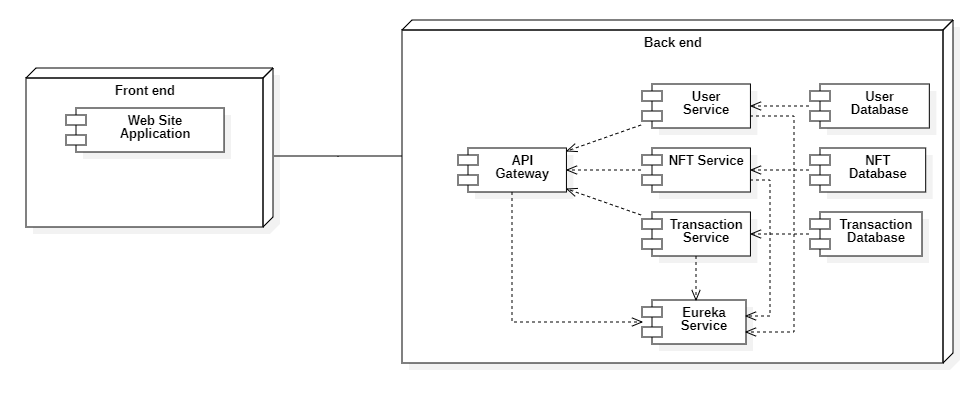
\includegraphics[scale=0.65]{./immagini/componentNFTLab.png}
		\caption{Diagramma UML dei componenti del back-end}
	\end{figure}
\end{center}
Il back-end sviluppato per il progetto è composto da cinque servizi, due di supporto (eureka e gateway) e tre per le funzionalità richieste. \\
L'API che svolge la funzionalità di gateway crea al suo avvio le route di collegamento ai servizi User, NFT e Transaction. Questo routing permette di attuare richieste HTTP rivolgendosi solamente al gateway senza essere a conoscenza dell'indirizzo privato di ogni servizio. Il gateway si prenderà cura di instradare correttamente le richieste verso ogni servizio rispondendo al client con i dati ricevuti. Il framework Spring permette la creazione di API gateway attraverso il pacchetto Spring Cloud Gateway, usando questa libreria infatti sarà solo necessario impostare le proprietà del file \emph{application.properties} e inserire la dipendenza nel file pom.xml per utilizzare tutte le sue funzionalità.

Una volta completati i due passaggi appena spiegati è necessario solo creare le route all'interno del controller dell'applicativo e l'autoconfigurazione di Spring si occuperà di generare le componenti autonomamente.
\\
Il servizio eureka invece è stato sviluppato usando il framework Spring Cloud Netflix che permette un'autoconfigurazione completa del servizio impostando solamente l'\emph{application.properties} e inserendo l'annotazione \emph{@EnableEurekaServer} nel file main del progetto Java.

I tre servizi che espongono le funzionalità del prodotto da sviluppare sono collegati a tre database diversi secondo l'architettura a microservizi. I database sono stati creati usando MySQL implementato dal programma XAMPP. 
\section{Struttura generale dei servizi}
Ogni servizio è composto dai tre livelli del pattern MVC: Presentation Layer, Business Logic Layer e Data Layer. Il Presentatio Layer viene definito nel package Controller, il controller definisce l'interfaccia con l'esterno e con la quale si può interagire con l'applicativo. Il Business Logic Layer viene definito nel package Service, in esso vengono manipolati i dati e formulate le risposte per ogni richiesta. Infine il Data Layer è definito attraverso il package Repository e il package dei modelli degli oggetti (User, Opera, Transaction etc), il repository è la classe che crea un collegamento al database attraverso i modelli degli oggetti creati utilizzando delle specifiche annotazioni, in questa classe possono essere definite query personalizzate oltre a quelle disponibili di default dal framework Spring Data JPA. Il package con al suo interno i modelli degli oggetti invece serve esclusivamente per la definizione delle entità.
